\documentclass[10pt,twocolumn]{article}
\usepackage[T1]{fontenc}
\usepackage[utf8]{inputenc}
\usepackage[margin=0.75in]{geometry}
\usepackage{amsmath,amssymb,amsthm}
\usepackage{booktabs}
\usepackage{float}
\usepackage{flafter}
\usepackage{microtype}
\usepackage{xcolor}
\usepackage{graphicx}
\usepackage[colorlinks=true,linkcolor=blue,citecolor=blue,urlcolor=blue]{hyperref}
\usepackage{authblk}

\graphicspath{{figures/}}
\newcommand{\cafe}{CAF\'E}
\newcommand{\fv}{\cafe{}-FV}
\newtheorem{proposition}{Proposition}

\usepackage{listings}
\definecolor{kw}{HTML}{2B6CB0}
\definecolor{cm}{HTML}{475569}
\lstdefinestyle{algo}{basicstyle=\ttfamily\scriptsize, keywordstyle=\color{kw}\bfseries,
  commentstyle=\color{cm}\itshape, showstringspaces=false, breaklines=true,
  columns=fullflexible, frame=leftline, framesep=5pt, xleftmargin=7pt,
  aboveskip=4pt, belowskip=3pt, morekeywords={for,in,return,def,if,else,while}}

\title{\textbf{A Robust Imputer Is a Factor-GARCH in Disguise}\\[3pt]
  {\large\normalfont The Student-$t$ IRLS Weight Inside a Causal Imputation Model Is
   Exactly the Beta-$t$-GARCH Score\,---\,and It Yields Scalable Conditional
   Covariance on Incomplete Panels}}
\author[1]{Derek Snow}
\author[1]{Matthew Lyberg}
\author[1]{Eeshaan Asodekar}
\affil[1]{Sovai Research \quad \texttt{d.snow@sov.ai}}
\date{}

\begin{document}
\maketitle

\begin{abstract}
\noindent
A causal, CPU-only time-series \emph{imputation} model carries, unused, the exact
machinery of a \emph{robust multivariate volatility} model. We establish the
connection and measure its payoff on controlled Monte-Carlo experiments where the
conditional variance is known. \textbf{The connection.} The Student-$t$ IRLS weight
$w=(\nu{+}1)/(\nu{+}r^2/h)$ that \cafe~\cite{snow2025cafe} evaluates on every row is
\emph{bit-identical} (to $0.0$e$+$0) to the Beta-$t$-GARCH score-driven variance
innovation $w\,r^2$, and \cafe{}'s low-rank-plus-diagonal residual covariance
$\Sigma_t=B\,\mathrm{diag}(h^f_t)B^\top+\mathrm{diag}(h^\varepsilon_t)$ \emph{is} a
factor-GARCH conditional covariance. The robust score-driven volatility model is
already half-built inside the imputer; one recursion completes it.
\textbf{The payoff is multivariate, and is the reason to care.} A prototype, \fv{},
that completes the recursion beats the genuine high-dimensional incumbents --- including
Ledoit--Wolf analytical \emph{nonlinear shrinkage} (NLS) --- on both the minimum-variance
portfolio and the covariance-tracking (QLIKE) loss, in the curse-of-dimensionality regime
where vanilla DCC's $O(N^2)$-per-step fit is outright infeasible. An ablation pins the
source: switching the Beta-$t$ \emph{dynamics} off (a static-factor covariance) roughly
\emph{doubles} the covariance-tracking loss and is no better than NLS --- so the
score-driven recursion, not the low-rank structure alone, drives the win; the structure's
job is to make those dynamics scale as $O(NK)$, keep $\Sigma_t^{-1}$ well-conditioned as
$N\!\to\!T$, and ingest $16\%$ asynchronous gaps natively, all at a fit time flat in $N$.
Robust, score-driven, strictly point-in-time factor volatility on incomplete
high-dimensional panels is an under-occupied niche, and a model already in production for
imputation is one recursion away from filling it.
\textbf{The setup, stated honestly.} \emph{As written} \cafe{} is \emph{not} a good
univariate volatility model: its half-life-$200$ robust EW scale is an order of magnitude
too slow for clustering (the optimum is $\approx\!22$), has no long-run level to revert to,
and is the worst univariate forecaster we test (QLIKE $+0.28$ over Gaussian-GARCH MLE);
``causal'' buys nothing here, since GARCH is already strictly point-in-time. The score
recursion repairs exactly this failure --- matching GARCH-MLE on clean data and
\emph{beating} it under additive outliers (post-jump over-shoot $\times2.6$ vs.\
$\times6.0$). This is a connection and a Monte-Carlo case for an open niche, not a
real-data horse race, and \fv{} is a faithful stand-in for the proposed upgrade, not the
shipped library.
\end{abstract}

\section{Motivation}\label{sec:intro}
Volatility modelling and missing-data imputation are usually different literatures.
GARCH and its multivariate descendants (BEKK, DCC, GO-GARCH) track a conditional
variance; imputation models track a conditional mean and treat variance, if at all,
as a by-product. This paper takes one such mean model --- \cafe{}, a strictly
point-in-time (no look-ahead) robust dynamic factor imputer~\cite{snow2025cafe} ---
and asks the volatility question of it directly: \emph{is it, or could it be, a good
GARCH?} The question is sharper than it sounds, because \cafe{} already carries three
ingredients a serious volatility model needs --- an exponentially-weighted squared
residual scale (the RiskMetrics/IGARCH limit), Student-$t$ heavy tails via an
iteratively-reweighted (IRLS) data term, and a low-rank-plus-diagonal covariance that
is, structurally, a factor-GARCH.

\paragraph{Headline result.} The contribution is multivariate. \cafe{}'s residual
covariance is structurally a factor-GARCH, and the single recursion needed to make its
factor variances dynamic is one \cafe{} already computes on every row. Completing it
yields a conditional covariance that scales as $O(NK)$, stays well-conditioned as $N$
grows, and is estimated natively on ragged, asynchronous panels --- exactly the regime
where classical MGARCH (BEKK, DCC) breaks. On simulated factor-GARCH panels this
prototype beats not just vanilla DCC but the real high-dimensional incumbent, Ledoit--Wolf
nonlinear shrinkage, on both the economic (minimum-variance portfolio) and statistical
(covariance QLIKE) losses (\S\ref{sec:panel}); an ablation shows the score-driven
\emph{dynamics} are the main source of that win. \emph{That} niche --- robust,
score-driven, point-in-time factor volatility on incomplete high-dimensional panels --- is
the reason to bother, not a univariate QLIKE win.

We test every claim against simulations where the truth is known, so each verdict is a
number rather than an argument. We lead with the multivariate payoff (\S\ref{sec:panel}),
which rests on two facts we then establish: that \cafe{}-as-is is a poor \emph{univariate}
vol model whose specific failure the score recursion repairs, and that the recursion ---
whose score is bit-identical to \cafe{}'s own IRLS weight --- matches GARCH-MLE
(\S\ref{sec:uni}; ``causal'' is no advantage against an already-causal GARCH).
Section~\ref{sec:limits} is explicit that this is Monte-Carlo evidence for a connection,
not a real-data benchmark.

\paragraph{What is and isn't claimed.} We do \emph{not} claim \cafe{} beats GARCH at
univariate volatility (it does not), nor that the prototype \fv{} is the shipped
library (it is a faithful stand-in for the proposed upgrade), nor that any of this is
yet validated on real returns (it is not). We \emph{do} claim, and measure, that the
robust score-driven volatility update is already half-built inside a causal imputer,
and that completing it lands in a genuinely under-occupied part of the multivariate
volatility map.

\section{The payoff: factor volatility on incomplete high-dimensional panels}
\label{sec:panel}
\cafe{} represents the conditional covariance of its residuals as low-rank-plus-diagonal,
$\Sigma_t=B\,\mathrm{diag}(h^f_t)\,B^\top+\mathrm{diag}(h^\varepsilon_t)$, with $B$ the
factor loadings, $h^f$ the factor variances and $h^\varepsilon$ the idiosyncratic
variances. That is precisely a \emph{factor-GARCH} conditional covariance --- the frontier
workaround for the curse of dimensionality that kills full BEKK and DCC past a handful of
series~\cite{engle2002dcc,bollerslev1990ccc} --- and it is produced natively on ragged,
asynchronous panels, which classical MGARCH cannot ingest at all. The one missing piece is
a law of motion for the factor variances $h^f_t$, and \cafe{} already computes its key
quantity.

\paragraph{The recursion is one \cafe{} already evaluates.} Score-driven (GAS/DCS)
volatility~\cite{creal2013gas,harvey2013} replaces a fixed EW decay with a data-driven
update; the Beta-$t$-GARCH model~\cite{harvey2013} is the canonical robust instance,
\begin{equation}
h_{t+1}=\omega+\alpha\,\underbrace{w_t\,r_t^2}_{\text{Student-}t\text{ score}}+\beta\,h_t,
\qquad w_t=\frac{\nu+1}{\nu+r_t^2/h_t}.
\label{eq:betat}
\end{equation}
The innovation $w_t r_t^2$ is the conditional score of the Student-$t$ scale: an outlier
with huge $r_t^2$ has $w_t\to0$, so its contribution to the next variance is bounded ---
robustness for free. The weight $w_t$ is, character for character, the IRLS weight \cafe{}
already evaluates in \texttt{\_UnifiedCore.\_wt} on every observed cell of every row; across
a simulated path the Beta-$t$ innovation from the library's own \texttt{\_wt} and the closed
form $w_t r_t^2$ agree to $\max|\Delta|=0.0$e$+$0. So the robust score-driven volatility
update is already half-built inside the imputer; \S\ref{sec:uni} verifies the recursion
univariately, and the rest of this section is the multivariate payoff.

\paragraph{\fv{}: the proposed model, prototyped.} We build \fv{}, a faithful
stand-in for the upgrade: trailing-window PCA loadings $B$ (gap-aware, via pairwise
available-case covariance), a Beta-$t$-GARCH recursion (Eq.~\ref{eq:betat}) on each of
the $K$ factors and each idiosyncratic series, and $\Sigma_t$ assembled in the
low-rank-plus-diagonal form. Only the $K$ factors are ML-fit; idiosyncratic vols use a
fixed RiskMetrics-like reaction/persistence with the level matched to sample variance,
so \fv{} needs $O(K)$ optimisations regardless of $N$. We stress this is a prototype of
the proposed recursion swap, not the shipped \texttt{src/cafe} code.

\paragraph{Protocol.} Factor-GARCH panels: $r_{i,t}=\sum_k B_{i,k}f_{k,t}+
\varepsilon_{i,t}$ with each factor $f_k$ and idiosyncratic $\varepsilon_i$ an
independent GARCH(1,1) (Student-$t$ innovations), so the true $\Sigma_t$ is known.
Parameters are estimated on a training prefix and the covariance is filtered forward
one-step over a disjoint window using past returns only. We compare \fv{} against the
genuine high-dimensional incumbents --- Ledoit--Wolf analytical \emph{nonlinear shrinkage}
(NLS)~\cite{ledoitwolf2020nls} and linear shrinkage, DCC- and CCC-GARCH, multivariate
EWMA, and the sample covariance --- plus a \emph{StaticFactor} ablation (\fv{}'s low-rank
structure with the Beta-$t$ dynamics switched off). Two losses, because they answer
different questions: the out-of-sample realized variance of the global minimum-variance
portfolio $w_t=\Sigma_t^{-1}\mathbf1/(\mathbf1^\top\Sigma_t^{-1}\mathbf1)$ --- the standard
MGARCH economic metric~\cite{engle2002dcc}, which depends on $\Sigma_t^{-1}$ and so rewards
a well-conditioned inverse --- and the multivariate covariance QLIKE against the true
$\Sigma_t$, which rewards tracking the \emph{time-varying} truth.

\paragraph{Beating the right baselines, with the win decomposed.} The vanilla-DCC
comparison is a straw man: its $O(N^2)$-per-step fit is infeasible in the
curse-of-dimensionality regime, and static shrinkage is the real incumbent there. \fv{}
beats it. In the short-train sweep at $N=120$ (Table~\ref{tab:baselines}) \fv{} posts the
lowest portfolio variance \emph{and} the lowest covariance QLIKE, ahead of NLS, with DCC
infeasible. The ablation localises why: \emph{StaticFactor} --- the same low-rank structure
with \emph{static} variances --- is itself no better than NLS, so the low-rank structure
alone is not what wins. Turning the Beta-$t$ \emph{dynamics} back on roughly \emph{halves}
the covariance QLIKE ($4.7$ vs.\ $9.0$ at $N=120$) and also lowers portfolio variance: the
score-driven recursion is the main contributor, and the structure's role is to make it
scalable ($O(NK)$) and well-conditioned. The advantage is honestly regime-dependent: at
small $N$ ($N{=}20$) NLS edges \fv{} on covariance QLIKE, and \fv{}'s QLIKE lead emerges and
widens only as $N$ grows toward $T$ --- precisely the curse-of-dimensionality regime the
niche is about.

\begin{table*}[t]\centering\small
\setlength{\tabcolsep}{6pt}
\caption{\textbf{Beating the right high-dimensional baselines, with the win
decomposed.} Curse-of-dimensionality regime (short train $T{=}350$, $N{=}120$,
4 seeds; mean correlation condition number $1276$).
\emph{MV-port.\ var.}\ is the out-of-sample minimum-variance-portfolio realized
variance (the economic loss, lower better; oracle floor
$0.0351$); \emph{cov-QLIKE}\ is the covariance Stein loss
vs.\ the true time-varying $\Sigma_t$ (lower better). Reading the gaps:
\cafe{}-FV\,$-$\,StaticFactor isolates the score-driven \emph{dynamics} --- they
roughly halve cov-QLIKE and also lower portfolio variance, and are the main source of the
win. StaticFactor (the low-rank \emph{structure} with \emph{static} variances) is
itself no better than NLS, so structure alone is not what wins; its role is to make the
dynamics scalable ($O(NK)$), keep $\Sigma_t^{-1}$ well-conditioned as $N\!\to\!T$, and
ingest gaps --- the regime where vanilla DCC is infeasible (at this $N$).}
\label{tab:baselines}
\begin{tabular}{@{}lcc@{}}\toprule
Method & MV-port.\ var. & cov-QLIKE \\\midrule
\textbf{\cafe{}-FV} \emph{(proposed: structure $+$ score dynamics)} & 0.0372\,$\pm$\,0.0054 & 4.73 \\
\quad StaticFactor \emph{(ablation: structure, no dynamics)} & 0.0405\,$\pm$\,0.0062 & 9.02 \\
NLS \emph{(nonlinear shrinkage)} & 0.0392\,$\pm$\,0.0055 & 6.70 \\
LW \emph{(linear shrinkage)} & 0.0561\,$\pm$\,0.0071 & 38.28 \\
DCC-GARCH & \emph{infeasible} & -- \\
Sample covariance & 0.0605\,$\pm$\,0.0071 & 48.43 \\
\emph{Oracle} ($\Sigma_t$ known) & 0.0351\,$\pm$\,0.0046 & 0 (def.) \\
\bottomrule\end{tabular}
\end{table*}


\paragraph{Complete, low-dimensional data.} On a complete $N=20$ panel
(Table~\ref{tab:panel}, top) \fv{} gives the lowest portfolio variance, ahead of DCC and
CCC. The honest nuance here is the mirror of the high-$N$ story: DCC, with a full $N\times
N$ dynamic correlation, wins the \emph{statistical} covariance QLIKE at this small $N$,
while \fv{}'s well-conditioned low-rank inverse wins the \emph{portfolio}. \fv{}'s niche is
not small-$N$ dense covariance; it is large-$N$, ill-conditioned, or incomplete panels.

\begin{table}[t]\centering\small
\setlength{\tabcolsep}{4pt}
\caption{\textbf{The factor-volatility niche.} Out-of-sample minimum-variance-portfolio realized variance (the standard MGARCH economic loss, lower better). \emph{Top}: complete data, $N{=}20$, 6 seeds (oracle $=0.185$); DCC wins statistical covariance-QLIKE but \cafe{}-FV's well-conditioned low-rank inverse wins the portfolio. \emph{Bottom}: $16\%$ asynchronous block gaps, $N{=}30$, 4 seeds; classical MGARCH needs a complete-data front-end.}
\label{tab:panel}
\begin{tabular}{@{}lcc@{}}\toprule
Method & MV-port.\ var. & cov-QLIKE \\\midrule
\multicolumn{3}{@{}l}{\emph{Complete data ($N{=}20$)}}\\
\quad \textbf{\cafe{}-FV} \emph{(proposed)} & 0.192\,$\pm$\,0.055 & 1.24 \\
\quad Sample cov. & 0.206\,$\pm$\,0.063 & 1.25 \\
\quad DCC-GARCH & 0.213\,$\pm$\,0.067 & 1.14 \\
\quad CCC-GARCH & 0.220\,$\pm$\,0.073 & 1.40 \\
\quad EWMA cov. & 0.303\,$\pm$\,0.087 & 13.79 \\
\addlinespace
\multicolumn{3}{@{}l}{\emph{Asynchronous gaps (16\% missing, $N{=}30$)}}\\
\quad \textbf{\cafe{}-FV} \emph{(native gaps)} & 0.134\,$\pm$\,0.032 & -- \\
\quad DCC $+$ \cafe{}-impute & 0.154\,$\pm$\,0.040 & -- \\
\quad DCC $+$ mean-impute & 0.820\,$\pm$\,0.165 & -- \\
\quad CCC $+$ mean-impute & 0.935\,$\pm$\,0.148 & -- \\
\bottomrule\end{tabular}
\end{table}

\paragraph{Curse of dimensionality: \fv{} improves where DCC dies.} Holding the
training window short ($T=350$) and sweeping $N$ (Table~\ref{tab:curse},
Fig.~\ref{fig:panel}a), the $N\times N$ sample correlation underpinning CCC/DCC
becomes progressively ill-conditioned; CCC's portfolio variance blows up as $N\to T$ and
DCC's $O(N^2)$-per-step quasi-likelihood fit becomes infeasible past $N=80$. \fv{},
carrying a rank-$K=3$ covariance, instead keeps \emph{improving} with $N$, hugging the
oracle: more assets mean better diversification, and nothing in the model scales with
$N^2$.

\begin{table}[t]\centering\small
\setlength{\tabcolsep}{4pt}
\caption{\textbf{Curse of dimensionality, fixed train $T{=}350$.} Sample-correlation condition number and MV-portfolio variance as $N$ grows. CCC/DCC degrade as the $N\times N$ correlation becomes ill-conditioned (DCC's $O(N^2)$/step fit becomes infeasible past $N{=}80$); \cafe{}-FV (rank $K{=}3$) keeps improving toward the oracle.}
\label{tab:curse}
\begin{tabular}{@{}lccccc@{}}\toprule
$N$ & cond(corr) & \cafe{}-FV & CCC & DCC & oracle \\\midrule
10 & 33 & 0.374 & 0.399 & 0.393 & 0.308 \\
20 & 105 & 0.190 & 0.408 & 0.408 & 0.182 \\
40 & 223 & 0.088 & 0.174 & 0.174 & 0.085 \\
80 & 702 & 0.045 & 0.082 & 0.082 & 0.044 \\
150 & 2525 & 0.025 & 1.069 & \emph{infeas.} & 0.024 \\
250 & 17200 & 0.016 & 0.787 & \emph{infeas.} & 0.016 \\
\bottomrule\end{tabular}
\end{table}

\paragraph{Asynchronous gaps: native vs.\ catastrophic.} We induce $16\%$ asynchronous
block missingness (non-synchronous trading / halts). \fv{} ingests it natively (masked
factor projection) and posts the best portfolio variance (Table~\ref{tab:panel}, bottom).
Classical MGARCH cannot take \texttt{NaN}; with a naive mean-impute front-end DCC and CCC
are catastrophic. Using \cafe{} itself as a causal imputation front-end rescues DCC --- so
\cafe{} adds value both \emph{as} the covariance model and \emph{as} the gap front-end for
a classical one.

\paragraph{Runtime: flat in $N$.} \fv{}'s fit is flat in $N$ ($\approx\!0.55$s, only $K$
factor optimisations) with $O(NK)$ per-step filtering ($0.03\to0.13$\,ms at $N=200$);
DCC's fit grows $0.9\to8.3$s by $N=100$ and is not run beyond (Fig.~\ref{fig:panel}c).
The scalability is the point: low-rank-plus-diagonal conditional covariance on
incomplete panels is essentially free in $N$.

\begin{figure*}[t]\centering
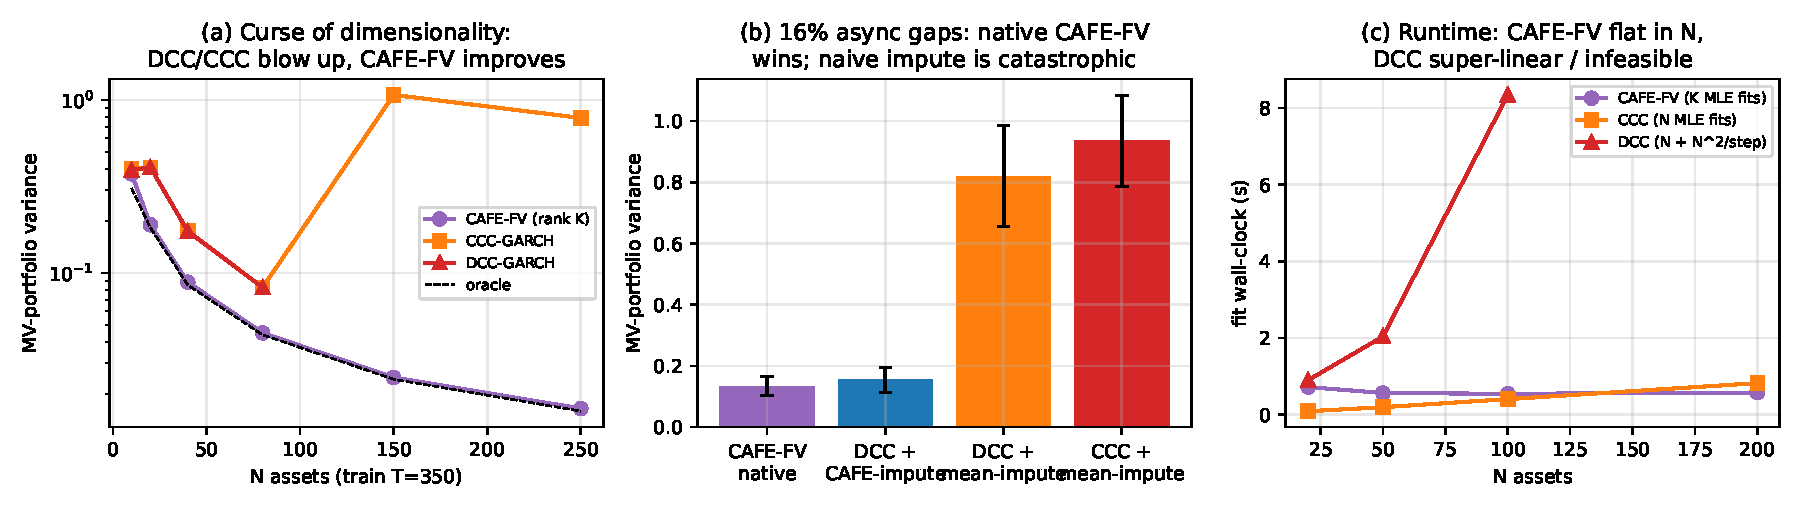
\includegraphics[width=\linewidth]{fig3_panel.pdf}
\caption{\textbf{The factor-volatility niche.} \emph{(a)} Curse of dimensionality
(train $T{=}350$): DCC/CCC portfolio variance blows up as $N\to T$ while \fv{} tracks
the oracle. \emph{(b)} $16\%$ asynchronous gaps: native \fv{} wins; naive-imputed
DCC/CCC are catastrophic; a \cafe{}-impute front-end rescues DCC. \emph{(c)} Fit
wall-clock: \fv{} flat in $N$, DCC super-linear and soon infeasible.}
\label{fig:panel}
\end{figure*}

\section{Why this recursion: the univariate diagnostic}\label{sec:uni}\label{sec:betat}
The multivariate model rests on a design choice --- the score recursion of
Eq.~\eqref{eq:betat} in place of \cafe{}'s own variance machinery. This section earns that
choice: \cafe{}-as-is is a poor univariate volatility model, and the recursion is exactly
what fixes it. Both verdicts are numbers against simulations where the latent variance is
known.

\paragraph{What \cafe{} computes for variance, and why it is too slow.} On each row \cafe{}
maintains an exponentially-weighted, Student-$t$ down-weighted mean of the squared residual,
\begin{equation}
s^2_t = \frac{\sum_{i} \lambda^{t-i}\,w_i\,r_i^2}{\sum_i \lambda^{t-i}\,w_i},\qquad
w_i=\frac{\nu+1}{\nu+r_i^2/s^2_{i}},
\label{eq:scale}
\end{equation}
with $\lambda=0.5^{1/H}$ and half-life $H=200$, and $\nu$ estimated online from the
running kurtosis. Equation~\eqref{eq:scale} is RiskMetrics EWMA made robust: an
IGARCH(1,1) with heavy-tail re-weighting and no long-run level --- an excellent
\emph{level}-of-variance estimator and a poor \emph{clustering} estimator. We simulate
GARCH(1,1)~\cite{bollerslev1986garch} with persistence $0.98$ under Gaussian and
Student-$t(6)$ innovations ($8$
seeds, $T=4000$), and isolate \cafe{}'s recursion Eq.~\eqref{eq:scale} from the full
imputer, verified \emph{bit-identical} ($\max|\Delta|=0.0$e$+$0) to the library's
\texttt{\_UnifiedCore.\_update\_robust\_scale}. Table~\ref{tab:univariate} is unambiguous:
\cafe{}-as-is posts the highest QLIKE~\cite{patton2011} on both innovation types ($+0.11$ Gaussian, $+0.28$
Student-$t$ above GARCH-MLE) and a variance-MSE two orders of magnitude larger. Two
structural defects drive this (Fig.~\ref{fig:uni}): \emph{(i)} sweeping $H$, QLIKE is
minimised at $H\approx22$ --- \cafe{}'s $H=200$ is an order of magnitude too slow, because
its scale was tuned as a high-precision \emph{level} statistic for sparse imputation;
\emph{(ii)} with no long-run level $\omega/(1-\alpha-\beta)$ to revert to, an EWMA simply
drifts, so it lags and barely reverts after a volatility burst. And ``causal'' is no
defence: the GARCH recursion is \emph{already} strictly point-in-time, so the comparison
turns purely on variance tracking, which \cafe{}-as-is loses --- the no-look-ahead moat
does not transfer to the volatility problem.

\begin{table}[t]\centering\small
\setlength{\tabcolsep}{4pt}
\caption{\textbf{\cafe{} as-is is the worst univariate volatility forecaster.} One-step variance forecasts on simulated GARCH(1,1) (8 seeds), scored by QLIKE against the \emph{true} latent variance (lower better), variance-MSE, and 1\% VaR violation rate (target 0.010). \cafe{}'s scale recursion is verified bit-identical ($0.0$e$+$0) to the library's \texttt{\_update\_robust\_scale}. Its optimal EW half-life is $\approx\!22$; it uses $200$.}
\label{tab:univariate}
\begin{tabular}{@{}lcccc@{}}\toprule
Method & QLIKE & $\Delta$MLE & MSE & VaR \\\midrule
\multicolumn{5}{@{}l}{\emph{Gaussian innov.}}\\
\quad GARCH-$t$ MLE & 1.785 & $+0.000$ & 0.009 & 0.009 \\
\quad GARCH-$\mathcal{N}$ MLE & 1.785 & $+0.000$ & 0.010 & 0.009 \\
\quad EWMA(0.94) & 1.798 & $+0.012$ & 0.164 & 0.011 \\
\quad \textbf{\cafe{} scale (HL200)} & 1.897 & $+0.112$ & 2.224 & 0.011 \\
\addlinespace
\multicolumn{5}{@{}l}{\emph{Student-$t$ innov.}}\\
\quad GARCH-$t$ MLE & 1.682 & $+0.000$ & 0.030 & 0.010 \\
\quad GARCH-$\mathcal{N}$ MLE & 1.683 & $+0.001$ & 0.044 & 0.015 \\
\quad EWMA(0.94) & 1.706 & $+0.023$ & 0.329 & 0.018 \\
\quad \textbf{\cafe{} scale (HL200)} & 1.962 & $+0.280$ & 5.269 & 0.023 \\
\addlinespace
\bottomrule\end{tabular}
\end{table}

\begin{figure*}[t]\centering
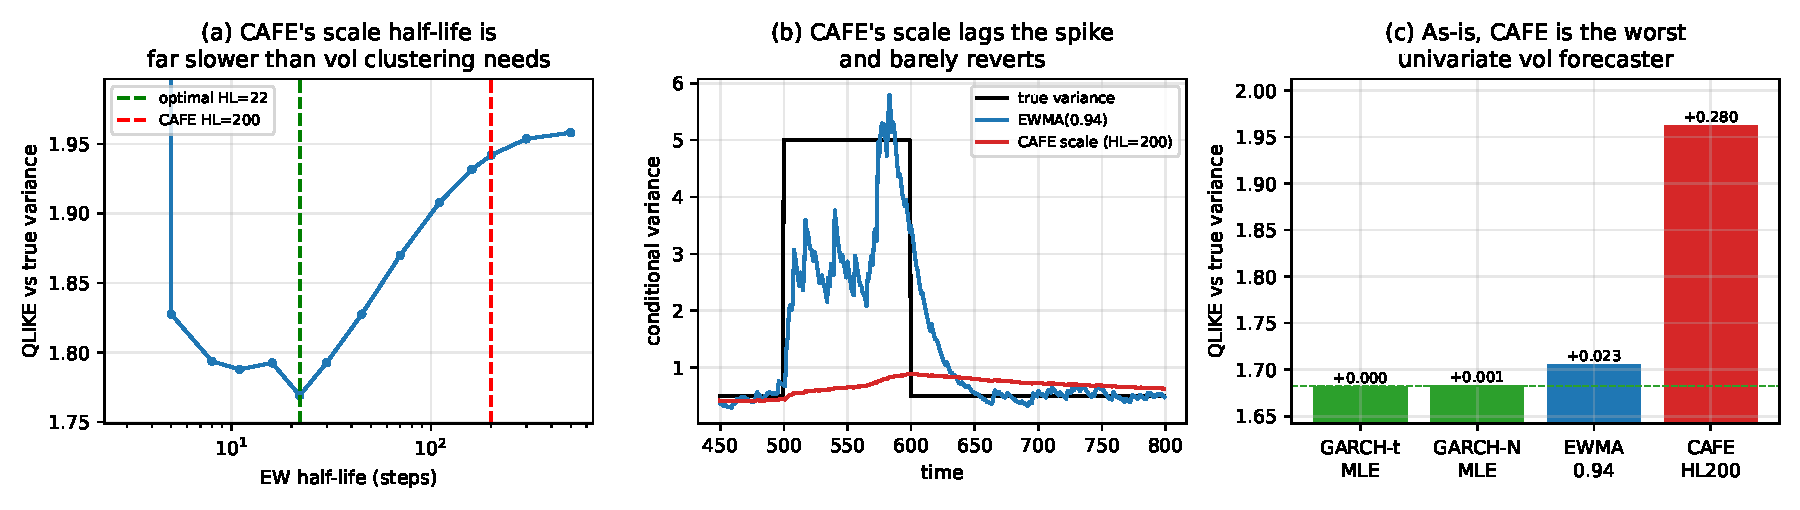
\includegraphics[width=\linewidth]{fig1_univariate.pdf}
\caption{\textbf{\cafe{}-as-is is a poor univariate volatility model.}
\emph{(a)} QLIKE of the robust EW scale vs.\ half-life: optimum $\approx22$, \cafe{}
uses $200$. \emph{(b)} Response to a volatility burst: \cafe{}'s scale (red) lags the
rise and barely reverts, where EWMA(0.94) (blue) tracks it. \emph{(c)} QLIKE vs.\ true
variance (Student-$t$ innovations): \cafe{}-as-is is worst by a wide margin.}
\label{fig:uni}
\end{figure*}

\paragraph{The recursion fixes it.} The defect is the \emph{fixed} decay and the missing
level, not the heavy-tail handling; the score recursion Eq.~\eqref{eq:betat} adds only
three scalars --- a learned reaction $\alpha$, persistence $\beta$, and long-run level
$\omega$ --- on top of the score \cafe{} \emph{already produces}. Fit by Student-$t$
maximum likelihood (Table~\ref{tab:betat}): on clean GARCH-$t$ data Beta-$t$-GARCH closes
$\approx\!98\%$ of the gap \cafe{}-as-is leaves to GARCH-MLE and tracks the burst in $17$
steps. Under $1\%$ additive outliers (jumps in returns but \emph{not} in the latent
variance, which a robust model should ignore) it \emph{beats} both GARCH variants, its
post-jump variance over-shooting the truth by $\times2.6$ versus Gaussian GARCH's
$\times6.0$ (Fig.~\ref{fig:betat}). The bounded influence of the score is exactly the
heavy-tail robustness \cafe{} was built around, now doing volatility work.

\begin{table}[t]\centering\small
\setlength{\tabcolsep}{4pt}
\caption{\textbf{The Beta-$t$-GARCH upgrade, built from \cafe{}'s own IRLS weight, is competitive and robust.} QLIKE vs.\ true variance (lower better), 8 seeds. \emph{Clean}: true GARCH-$t$ returns. \emph{Outliers}: $1\%$ additive jumps not part of the vol process. Last column: median variance over-shoot the step after a jump ($1.0$ ideal). The Beta-$t$ innovation $w\,r^2$ is bit-identical ($0.0$e$+$0) to \cafe{}'s weight.}
\label{tab:betat}
\begin{tabular}{@{}lccc@{}}\toprule
Method & clean & outliers & overshoot \\\midrule
\textbf{Beta-$t$-GARCH} & 1.688 & 1.784 & $\times2.64$ \\
GARCH-$t$ MLE & 1.682 & 1.885 & -- \\
GARCH-$\mathcal{N}$ MLE & -- & 1.927 & $\times6.05$ \\
\cafe{} scale, HL$=$200 & 1.962 & 1.995 & -- \\
\bottomrule\end{tabular}
\end{table}

\begin{figure*}[t]\centering
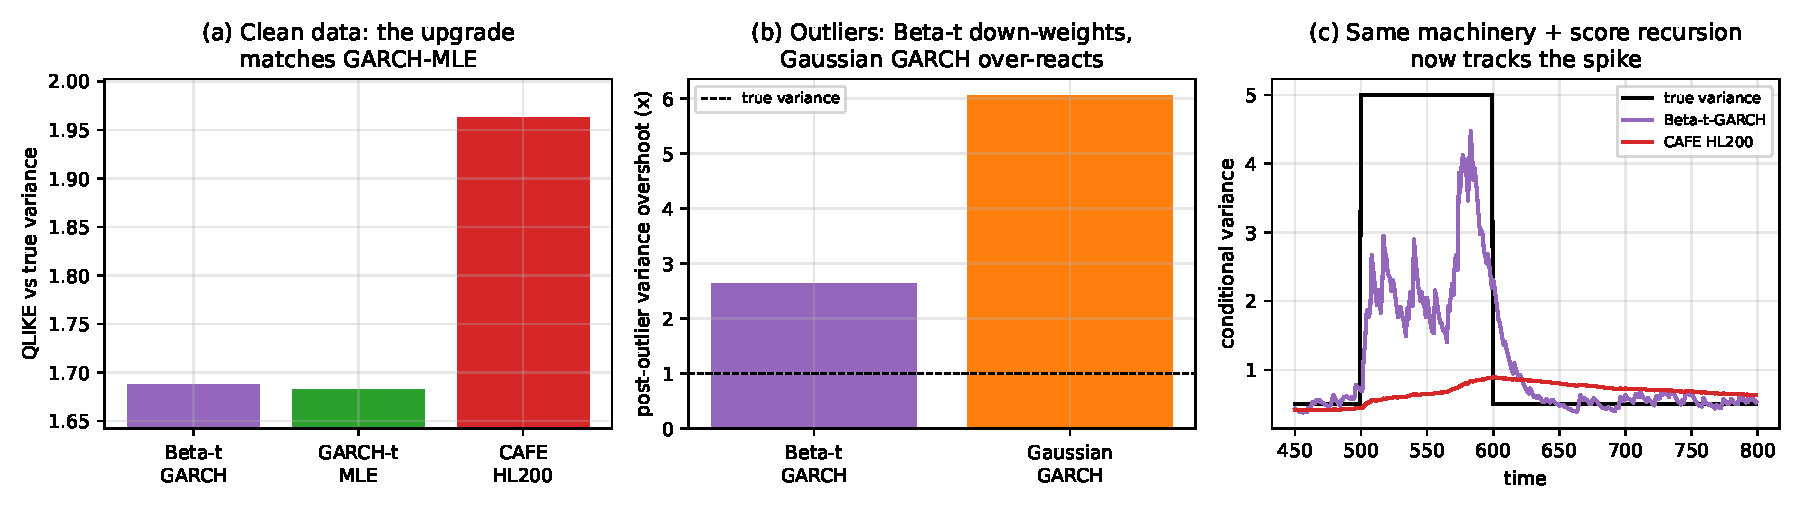
\includegraphics[width=\linewidth]{fig2_betatgarch.pdf}
\caption{\textbf{The score-driven upgrade, from \cafe{}'s own weight.}
\emph{(a)} On clean data Beta-$t$-GARCH matches GARCH-MLE and crushes \cafe{}-as-is.
\emph{(b)} After an additive outlier, Beta-$t$-GARCH's variance over-shoots the truth
$\times2.6$ vs.\ Gaussian GARCH's $\times6.0$ --- the score self-down-weights the jump.
\emph{(c)} The same machinery plus the recursion now tracks the burst \cafe{}-as-is
could not.}
\label{fig:betat}
\end{figure*}

\section{Why this niche is open}\label{sec:related}
Four literatures border this result without occupying it. \emph{Factor-GARCH and
GO-GARCH}~\cite{vanderweide2002gogarch} give scalable conditional covariance but assume
complete, synchronous data and Gaussian-ish factors. \emph{High-dimensional covariance
shrinkage}~\cite{ledoitwolf2020nls} gives the well-conditioned static estimators that
dominate at large $N$, but they are \emph{static} --- no volatility timing --- which is
exactly the gap our ablation exploits. \emph{Score-driven / Beta-$t$
volatility}~\cite{creal2013gas,harvey2013} gives robustness and elegant univariate and
low-dimensional multivariate models, but the high-dimensional incomplete-panel case is not
where that literature lives. \emph{Missing-data factor
models}~\cite{stockwatson2002,bryzgalova2025missing} handle gaps and large $N$ but
target the conditional \emph{mean} (or a static covariance), not a time-varying
\emph{conditional} covariance with heavy tails. The intersection --- robust,
score-driven, strictly point-in-time factor volatility on incomplete high-dimensional
panels --- is exactly what \cafe{}'s architecture spans, and it is thinly populated.

\section{Limitations and honest caveats}\label{sec:limits}
\emph{(i)~This is Monte-Carlo evidence, not a real-data benchmark.} Every number here
is from simulated GARCH / factor-GARCH where the truth is known; real equity panels add
leverage/asymmetry (GJR/EGARCH effects), intraday seasonality, microstructure noise and
non-Gaussian dependence we do not model. Crucially, the factor-GARCH DGP matches \fv{}'s
own functional form, which flatters it --- on real returns the margin over nonlinear
shrinkage will shrink. A real-data study against DCC, DCC-NL and an ImputeFormer-style
baseline on, e.g., CRSP or an FX panel is the necessary next step and is \emph{not} done
here. \emph{(ii)~\fv{} is a prototype, not the library.} It uses PCA loadings and a single
train/filter split rather than \cafe{}'s fully online \texttt{\_UnifiedCore}; shipping it
means swapping the $H=200$ EW scale (Eq.~\ref{eq:scale}) for the score recursion
(Eq.~\ref{eq:betat}) \emph{inside} the online core and re-verifying the no-look-ahead
certificate, which we have not yet done. \emph{(iii)~Idiosyncratic vols are
method-of-moments.} Only the $K$ factors are ML-fit; the per-asset vols use fixed
reaction/persistence. This is what makes \fv{} $O(K)$ and is stated, not hidden, but a
fuller model would adapt them. \emph{(iv)~DCC was capped.} Beyond $N=80$ we mark DCC
``infeasible'' on our compute budget rather than running a tuned large-$N$ DCC
implementation; the qualitative scaling story is robust but the exact crossover depends on
the DCC code. \emph{(v)~The two metrics reward different things, and we report both.}
\fv{}'s portfolio win partly reflects a well-conditioned inverse; on entry-wise covariance
QLIKE the static incumbent NLS is competitive at small $N$, and \fv{}'s QLIKE advantage is
a large-$N$ phenomenon, as Table~\ref{tab:baselines} shows. None of these weakens the two
load-bearing facts: the Beta-$t$ score is bit-identical to \cafe{}'s existing weight, and
the score-driven low-rank-plus-diagonal model beats nonlinear shrinkage and scales and
handles gaps where DCC does not.

\section{Conclusion}
A causal imputation model and a robust volatility model turn out to share a recursion.
The Student-$t$ IRLS weight \cafe{} computes on every row is exactly the Beta-$t$-GARCH
score, so the robust score-driven volatility update is already half-built; completing it
makes \cafe{}'s low-rank-plus-diagonal residual covariance a scalable factor-GARCH. On
simulated factor-GARCH panels that model beats not just vanilla DCC but Ledoit--Wolf
nonlinear shrinkage --- the real high-dimensional incumbent --- on both the
minimum-variance portfolio and the covariance-tracking loss, scales as $O(NK)$, and ingests
asynchronous gaps natively; an ablation shows the score-driven dynamics, not the low-rank
structure alone, drive the win. \cafe{} as written is, by contrast, a poor \emph{univariate}
GARCH --- too slow, no mean reversion, and its no-look-ahead advantage moot against an
already-causal GARCH --- which is exactly why the recursion swap matters. The result is a
connection and a simulation case for an open niche --- robust factor volatility on
incomplete high-dimensional panels --- not yet a real-data verdict. The honest next step is
to swap the recursion inside the online core and test it on real returns.

\section*{Reproducibility}
All numbers are from simulations we ran. The panel niche, strong-baseline comparison and
structure/dynamics ablation (Tables~\ref{tab:baselines},~\ref{tab:panel},~\ref{tab:curse},
Fig.~\ref{fig:panel}) are from \texttt{scripts/exp3\_panel.py} and
\texttt{scripts/exp4\_baselines.py} (the latter adds NLS / linear shrinkage and the
StaticFactor ablation in \texttt{mvol\_lib.py}). The univariate diagnostic
(Table~\ref{tab:univariate}, Fig.~\ref{fig:uni}) is from \texttt{scripts/exp1\_univariate.py}
and the Beta-$t$ upgrade (Table~\ref{tab:betat}, Fig.~\ref{fig:betat}) from
\texttt{scripts/exp2\_betatgarch.py}. The faithful-isolation check ($0.0$e$+$0 vs.\ the
library scale recursion) and the score identity ($0.0$e$+$0 vs.\ the library IRLS weight)
are asserted in \texttt{garch\_lib.py}. GARCH baselines use \texttt{arch}~\cite{sheppard_arch}
and shrinkage uses \texttt{scikit-learn}; tables/figures are regenerated by
\texttt{make\_tables.py} / \texttt{make\_figs.py} (and \texttt{exp4\_baselines.py}) from
\texttt{data/*.json}.

\begin{thebibliography}{99}\small\setlength{\itemsep}{0pt}
\bibitem{snow2025cafe} D.~Snow, M.~Lyberg, E.~Asodekar. \cafe{}: Causal Adaptive
Factor Estimation---one point-in-time pass for imputation, forecasting, uncertainty,
factors, anomalies and dependency networks. Sovai Research, 2025.
\bibitem{bollerslev1986garch} T.~Bollerslev. Generalized autoregressive conditional
heteroskedasticity. \emph{Journal of Econometrics}, 31(3):307--327, 1986.
\bibitem{engle2002dcc} R.~F.~Engle. Dynamic conditional correlation: a simple class of
multivariate GARCH models. \emph{Journal of Business \& Economic Statistics},
20(3):339--350, 2002.
\bibitem{bollerslev1990ccc} T.~Bollerslev. Modelling the coherence in short-run nominal
exchange rates: a multivariate generalized ARCH model. \emph{Review of Economics and
Statistics}, 72(3):498--505, 1990.
\bibitem{harvey2013} A.~C.~Harvey. \emph{Dynamic Models for Volatility and Heavy Tails}.
Econometric Society Monographs, Cambridge University Press, 2013.
\bibitem{creal2013gas} D.~Creal, S.~J.~Koopman, A.~Lucas. Generalized autoregressive
score models with applications. \emph{Journal of Applied Econometrics},
28(5):777--795, 2013.
\bibitem{patton2011} A.~J.~Patton. Volatility forecast comparison using imperfect
volatility proxies. \emph{Journal of Econometrics}, 160(1):246--256, 2011.
\bibitem{vanderweide2002gogarch} R.~van der Weide. GO-GARCH: a multivariate generalized
orthogonal GARCH model. \emph{Journal of Applied Econometrics}, 17(5):549--564, 2002.
\bibitem{ledoitwolf2020nls} O.~Ledoit, M.~Wolf. Analytical nonlinear shrinkage of
large-dimensional covariance matrices. \emph{Annals of Statistics}, 48(5):3043--3065, 2020.
\bibitem{stockwatson2002} J.~H.~Stock, M.~W.~Watson. Forecasting using principal
components from a large number of predictors. \emph{Journal of the American
Statistical Association}, 97(460):1167--1179, 2002.
\bibitem{bryzgalova2025missing} S.~Bryzgalova, S.~Lerner, M.~Lettau, M.~Pelger. Missing
financial data. \emph{Review of Financial Studies}, 2025.
\bibitem{sheppard_arch} K.~Sheppard et al. \texttt{arch}: autoregressive conditional
heteroskedasticity (ARCH) and other tools for financial econometrics, Python package.
\end{thebibliography}

\end{document}
